\chapter{Selection of Receiver Architecture}
\label{chap:rx}

A wide variety of different receiver designs exists each with it's advantages
and drawbacks. To come up with an optimal design, different receiver designs
were investigated using theoretical considerations and some were simulated to
further understand them. Thereby the focal point was on architectures we could
build in hardware using the Sivers IMA 58-63 GHz converter described in
\secref{sec:comp_sives}. \\

In the following chapters the terms \gls{TX} \gls{USBand} and \gls{TX}
\gls{LSBand} refere to the fact that the up-mixer used for transmitting
produces two signals at $f_{\text{TX LO}} \pm f_{\text{TX IF}}$ where
$f_{\text{TX LO}}$ is the frequency of the transmitters local oscillator
used for the mixer mixing to \gls{RF}. $f_{\text{TX IF}}$ is the central
frequency of the transmitters \gls{IF} signal. During all experiments
\gls{TX} \gls{USBand} was considered the desired signal and \gls{TX}
\gls{LSBand} a residual signal. \\

Analogous \gls{RX} \gls{USBand} and \gls{RX} \gls{LSBand} refere to
the down-mixer converting energy from $f_{\text{RX LO}} \pm f_{\text{RX IF}}$
to the same receiver \gls{IF} $f_{\text{RX IF}}$. \\

\section{Transmitter Architecture}
During this report always the same transmitter architecture was used.
It consists of two channel \gls{DAC} converting the $B = 1.8 \text{GHz}$ wide
\gls{TX} \gls{IF} signal at $f_{\text{TX IF}}$ and a $90^\circ$ phase shifted
version. \\

This two signals are than up-converter to
\gls{RF} and a $90^\circ$ coupler is used to suppress the \gls{LSBand}
as good as possible.
Therefor the \gls{USBand} considered the desired signal and the
not redidual \gls{LSBand} an interferer. \\

It was measured that in our setup the \gls{TX} \gls{LO} leackage
to the output \gls{RF} signal has similar power than the desired
signal it self. Therefor this leackage has to be considered and is
shown in all of the following spectrum drawing.
$f_{\text{TX IF}} = f_{\text{c}} - f_{\text{TX LO}}$ can be chosen accordingly
such that this leackage can be well enough suppressed. \\

Eventhough this would solve the problem of the the suppression of the
undesired \gls{TX} \gls{LO} leackage, in all receivers
$f_{\text{TX LO}}$ and $f_{\text{RX LO}}$ were choosen differently.
This was done to make sure that the residual \gls{TX} \gls{LSBand}
signal does not align with the desired \gls{TX} \gls{USBand} after
down-mixing. A perfekt alignment could result in an even better
\gls{SNR} due to the fact that additional signal energy is transmitted
alongside the desired \gls{TX} \gls{USBand} signal. \\

\section{RF Architecture}
All receivers have a band filter directely after the antenna simply by the
fact that all components (antenna, amplifiers, mixers etc.) have a frequency
selectivity which is often optimized only for the band of interest.
An additional band filter might be added to minimize the total power supplied
to the \gls{LNA} which has the main influence of the total noise figure of
the receiver. \\

Inside this band there are typically multiple channels with a carrier frequency
$f_c$ and a bandwidth $B$. \\

Since it is hard to build ajastable filters on \gls{RF} to select one specific
channel, this selection is typically done on an \gls{IF}. In our case of a
carrier frequency of $f_c \approx 60 \text{GHz}$ this \gls{IF} $f_{\text{IF}}$
is always lower than the carrier frequency $f_s$ due to component restrictions. \\

In the following two chapters two ways of building channel selection filters
are discussed. \\

\subsection{Image Rejection using high Intermediate Frequency}
\label{sec:rx_rf_0}
The mixer uses a \gls{LO} at $f_{\text{RX LO}}$ to mix the signal centered around
$f_{c}$ to an \gls{IF} of $f_{\text{RX IF}} = f_{c} - f_{\text{RX LO}}$. \\

The two signals $\pm (f_{c} + f_{\text{RX LO}})$ are not relevant since their
frequency is above 100 GHz and well beyond what the mixer output can drive. \\

$f_{\text{RX IF}}$ has to be high enough though such that the undesired
\gls{RX} \gls{LSBand} signal at $-f_{\text{c}} + f_{\text{RX LO}}$
does not convolve with the desired \gls{RX} \gls{USBand} signal.
This leads to a lower bound
$f_{\text{RX IF}} \geq B$ for the \gls{RX} \gls{IF} frequency
\footnote{%
  Infact $f_{\text{RX IF}} \geq \frac{B}{2}$
  is sufficient if later stages of the receiver can switch
  between \gls{USBand} and \gls{LSBand}.}. \\

A fixed channel filter is than used to suppress neighbouring channels
including the \gls{TX} \gls{LO} leackage witch was also mixed down. \\

\begin{figure}[ht]
  \centering
  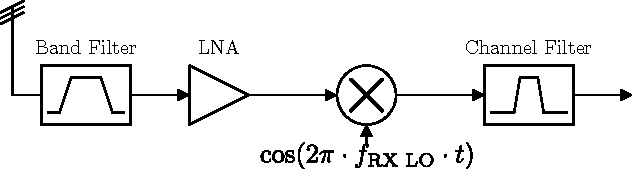
\includegraphics[width=\textwidth]{figures/rx_rf_0_bd}
  \caption{Block Diagram of Image Rejection using high \gls{IF}}
  \label{fig:rx_rf_0_bd}
\end{figure}

\subsection{Image Rejection using $90^\circ$ Couplers}
A second way to implement the suppression of the undesired \gls{RX}
\gls{LSBand} signal is to use $90^\circ$ couplers as described in
\secref{sec:comp_90deg}. \\

Lets assume we have the real \gls{RF} signal $s(t)$ shown in
\figref{fig:rx_rf_0_freq_s}.
The blue round signal centered around the carrier frequency $+f_c$ is our
desired signal and the spiky signal an undesired neighbouring channel.
Since it is a real signal, the negative frequencies consist of the mirrored,
complex conjugate signals which is painted in green. \\

By spliting it using a $90^\circ$ coupler we optain the two signals
$s(t)$ and $\mathcal{H}\{s(t)\}$ (drawn in \figref{fig:rx_rf_0_freq_Hs}).
$\mathcal{H}^{-1}$ denots the negative Hilbert transform which rotats the phase
of a signal by $-j$ for prositive and $j$ for negative frequencies
as shown in \figref{fig:hilbert}. \\

Next both signals are mixed by $f_{\text{RX LO}}$ resulting in two new signals
$a(t)$ and $b(t)$ as shown in \figref{fig:rx_rf_0_freq_a} and
\figref{fig:rx_rf_0_freq_b}.
The mirrors at $\pm (f_c + f_{\text{RX LO}})$ are already ignored. \\

By now using another $90^\circ$ coupler that applies the Hilbert transform
to $b(t)$ (drawn in \figref{fig:rx_rf_0_freq_Hb})
and adds $a(t)$ we end up with the real signal
$c(t) = a(t) + \mathcal{H}\{b(t)\}$
which is shown in \figref{fig:rx_rf_0_freq_c}. \\

One should note that the difference between $\mathcal{H}$ and $\mathcal{H}^{-1}$
is simply a swap of the two output plugs of a $90^\circ$ coupler since
the absolute phase reference is lost anyway. In fact both outputs are delayed
in time corresponding to negative phase rotation for positive frequencies
and a positive phase rotation for negative frequencies. \\

Finally a fixed channel selection filter can be used to at an arbitrary \gls{IF}
which is a clear advantage over the method discussed in \secref{sec:rx_rf_0}. \\

\begin{figure}[ht]
  \centering
  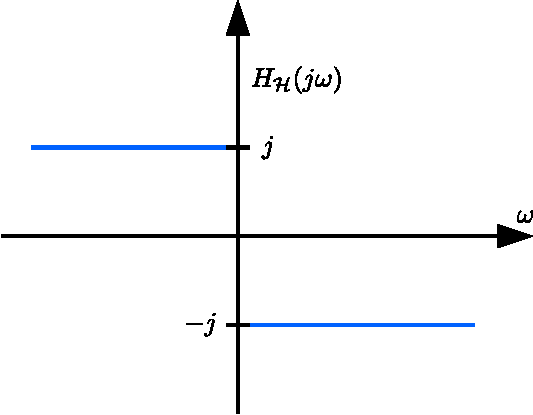
\includegraphics[width=0.3\textwidth]{figures/hilbert}
  \caption{Transfer Function of Hilbert Transform}
  \label{fig:hilbert}
\end{figure}

\begin{figure}[ht]
  \centering
  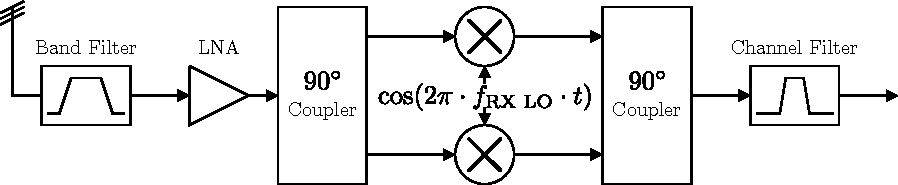
\includegraphics[width=\textwidth]{figures/rx_rf_1_bd}
  \caption{Block Diagram of Image Rejection using $90^\circ$ Couplers}
  \label{fig:rx_rf_0_bd}
\end{figure}

\begin{figure}[ht]
  \centering
  \begin{subfigure}{0.45\textwidth}
    \centering
    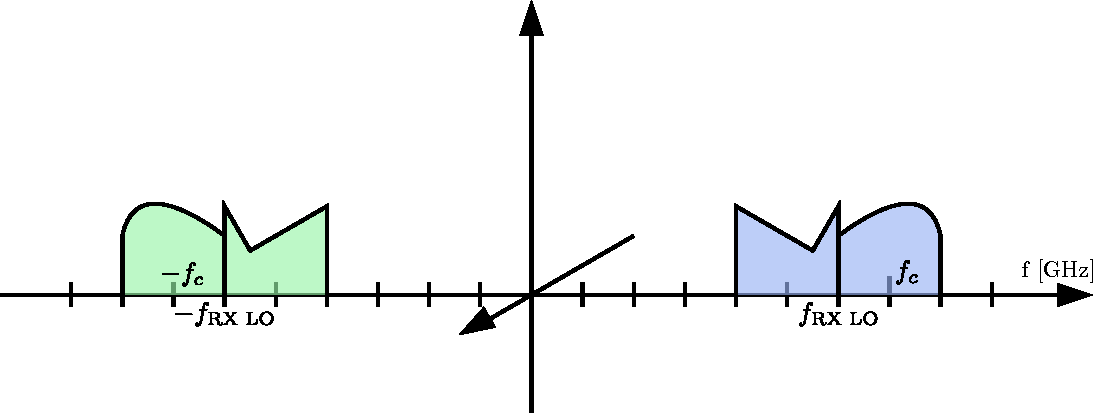
\includegraphics[width=\textwidth]{figures/rx_rf_0_freq_s}
    \caption{$s(t)$}
    \label{fig:rx_rf_0_freq_s}
  \end{subfigure}
  ~
  \begin{subfigure}{0.45\textwidth}
    \centering
    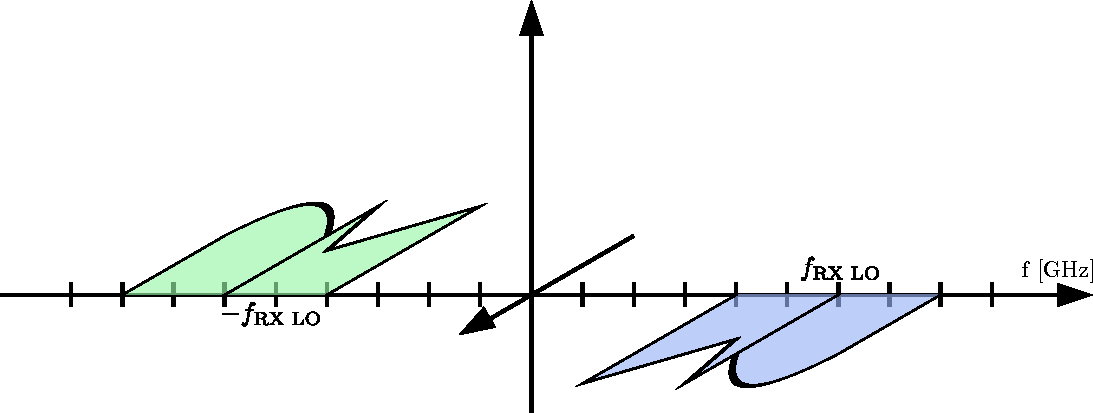
\includegraphics[width=\textwidth]{figures/rx_rf_0_freq_Hs}
    \caption{$\mathcal{H}^{-1}\{s(t)\}$}
    \label{fig:rx_rf_0_freq_Hs}
  \end{subfigure}
  \vspace{4ex} \\
  \begin{subfigure}{0.45\textwidth}
    \centering
    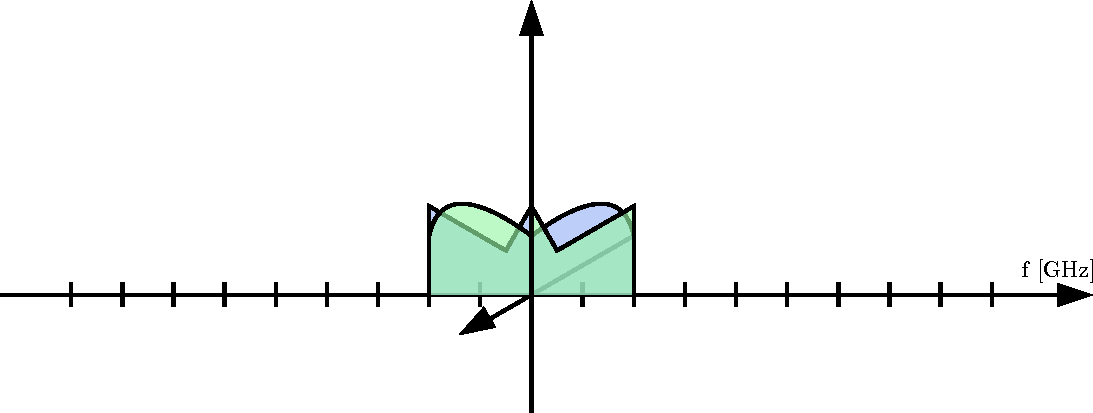
\includegraphics[width=\textwidth]{figures/rx_rf_0_freq_a}
    \caption{$a(t)$}
    \label{fig:rx_rf_0_freq_a}
  \end{subfigure}
  ~
  \begin{subfigure}{0.45\textwidth}
    \centering
    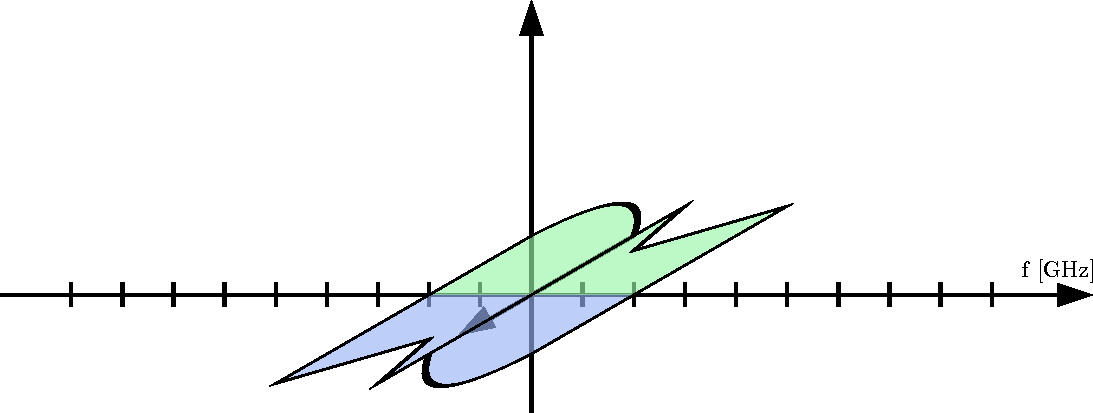
\includegraphics[width=\textwidth]{figures/rx_rf_0_freq_b}
    \caption{$b(t)$}
    \label{fig:rx_rf_0_freq_b}
  \end{subfigure}
  \vspace{4ex} \\
  \begin{subfigure}{0.45\textwidth}
    \centering
    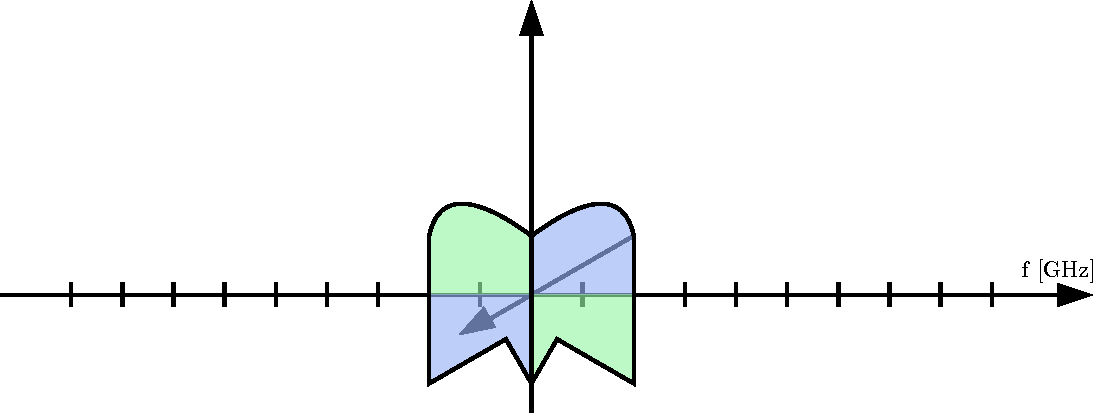
\includegraphics[width=\textwidth]{figures/rx_rf_0_freq_Hb}
    \caption{$\mathcal{H}^{-1}\{s(t)\}$}
    \label{fig:rx_rf_0_freq_Hb}
  \end{subfigure}
  ~
  \begin{subfigure}{0.45\textwidth}
    \centering
    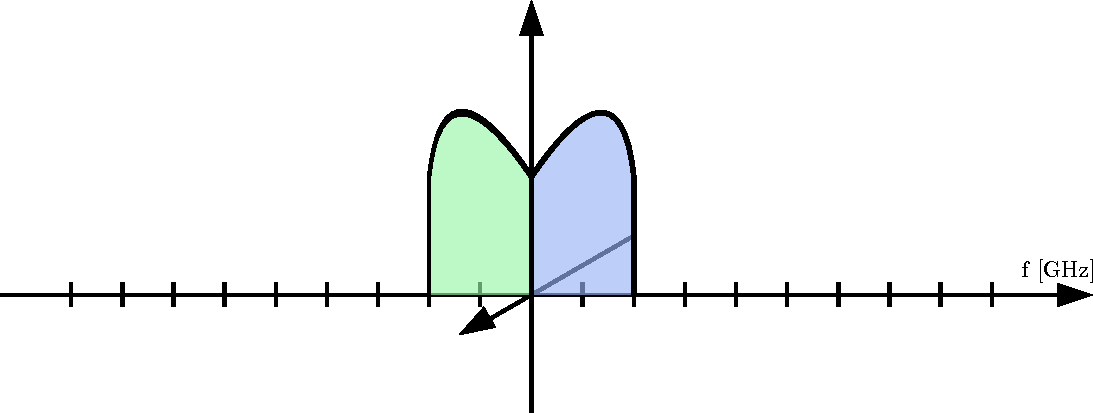
\includegraphics[width=\textwidth]{figures/rx_rf_0_freq_c}
    \caption{$c(t)$}
    \label{fig:rx_rf_0_freq_c}
  \end{subfigure}
  \caption{Image Rejection using $90^\circ$ Couplers}
  \label{fig:rx_rf_0_freq}
\end{figure}

\section{IF Architecture}
After the \gls{RF} part did the channel selection only the desired signal
is left and should be digitised.
This can be accomplished using different
mixing schemes of which three are shown in this section. \\

\subsection{Quadrature Baseband Sampling}
\label{sec:rx_adc_1}
The first \gls{IF} can be directly converted to baseband by
setting $f_{\text{LO}_2} = f_{\text{IF}}$.
Since our signal is assymetric the baseband signal is not analytic
and therefor quadrature sampling, which uses two mixers as shown in
\figref{fig:rx_adc_1_bd} is used. \\

Considering a \gls{IF} signal $i(t)$ (\figref{fig:rx_adc_1_freq_s})
with a center frequency of $f_{\text{IF}}$
and using the transformation \eqref{eq:four_cos} we can plot
$i(t)$ mixed with $\cos(2\pi \cdot f_{\text{IF}} \cdot t)$ as shown in
\figref{fig:rx_adc_1_freq_a}. \\

Analogous using \eqref{eq:four_sin} can be used to draw $i(t)$ mixed with
$\sin(2\pi \cdot f_{\text{IF}} \cdot t)$ as shown in
\figref{fig:rx_adc_1_freq_b}. \\

\begin{align}
  \label{eq:four_cos}
  \cos(\omega_0 \cdot t) \laplace \pi
  \left[\delta(\omega - \omega_0) - \delta(\omega + \omega_0) \right]
\end{align}

\begin{align}
  \label{eq:four_sin}
  \sin(\omega_0 \cdot t) \laplace \frac{\pi}{2}
  \left[\delta(\omega - \omega_0) + \delta(\omega + \omega_0) \right]
\end{align}

$a(t)$ and $b(t)$ are than low pass sampled to suppress the mirror image
at $2 f_{\text{IF}}$ and sampled by a two channel \gls{ADC} running with a
sample rate $f_s \geq B$. \\

Next the analytic signal $c(t)$ is constructed without any calculations
by simply interpreting the both \gls{ADC} channels as
$c(t) = a(t) + j \cdot b(t)$. To show that this works $j \cdot b(t)$
is plotted in \figref{fig:rx_adc_1_freq_jb} and
$c(t)$ in \figref{fig:rx_adc_1_freq_c}.

\begin{figure}[ht]
  \centering
  \begin{subfigure}{0.45\textwidth}
    \centering
    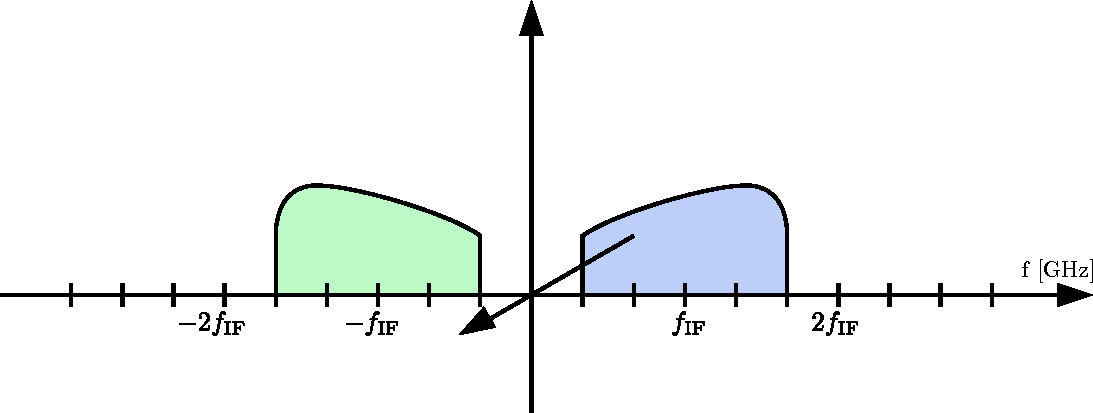
\includegraphics[width=\textwidth]{figures/rx_adc_1_freq_i}
    \caption{$i(t)$}
    \label{fig:rx_adc_1_freq_s}
  \end{subfigure}
  \vspace{4ex} \\
  \begin{subfigure}{0.45\textwidth}
    \centering
    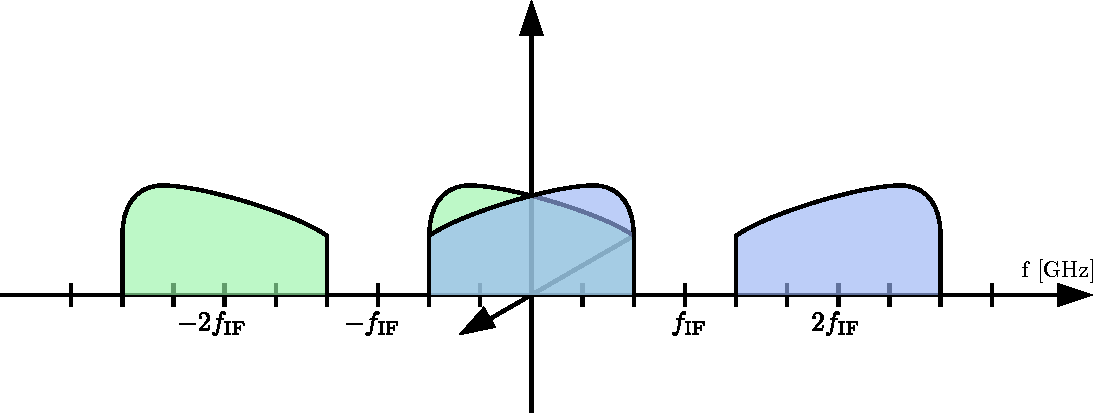
\includegraphics[width=\textwidth]{figures/rx_adc_1_freq_a}
    \caption{$a(t) = i(t) \cdot \cos(2\pi \cdot f_{\text{IF}} \cdot t)$}
    \label{fig:rx_adc_1_freq_a}
  \end{subfigure}
  ~
  \begin{subfigure}{0.45\textwidth}
    \centering
    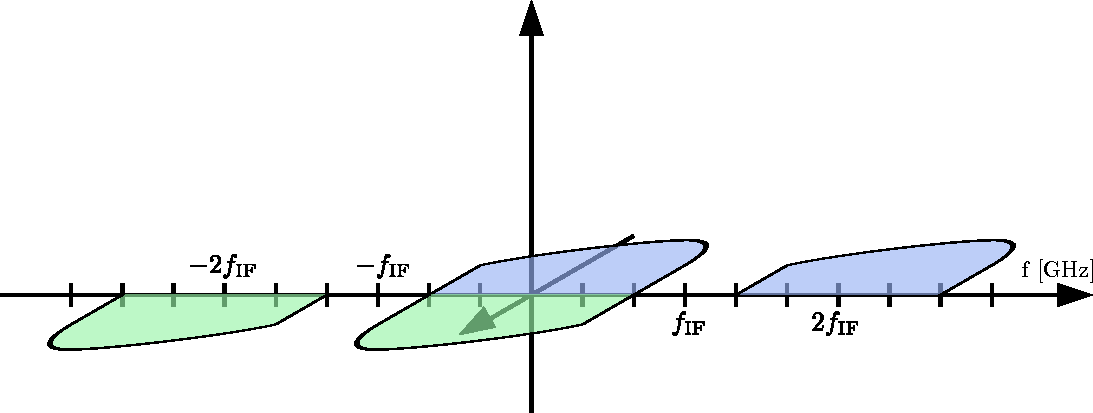
\includegraphics[width=\textwidth]{figures/rx_adc_1_freq_b}
    \caption{$b(t) = i(t) \cdot \sin(2\pi \cdot f_{\text{IF}} \cdot t)$}
    \label{fig:rx_adc_1_freq_b}
  \end{subfigure}
  \vspace{4ex} \\
  \begin{subfigure}{0.45\textwidth}
    \centering
    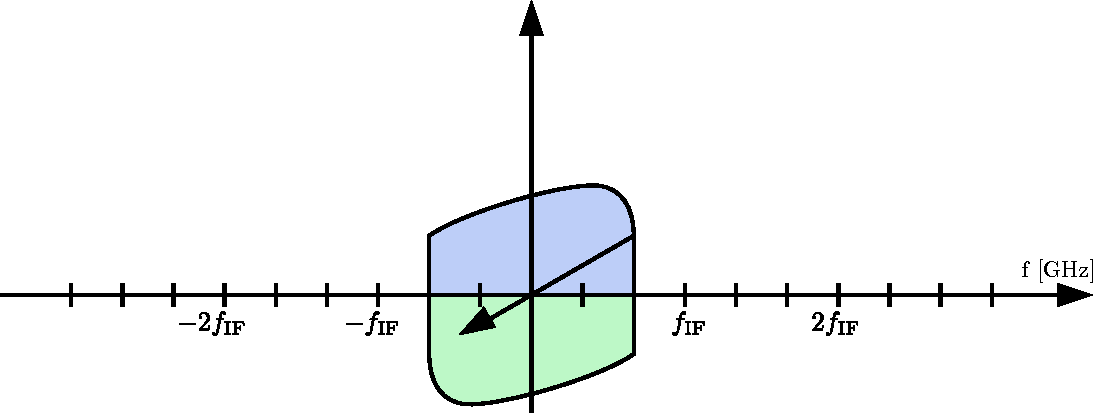
\includegraphics[width=\textwidth]{figures/rx_adc_1_freq_jb}
    \caption{$j \cdot \text{LP}\{b(t)\}$}
    \label{fig:rx_adc_1_freq_Hb}
  \end{subfigure}
  ~
  \begin{subfigure}{0.45\textwidth}
    \centering
    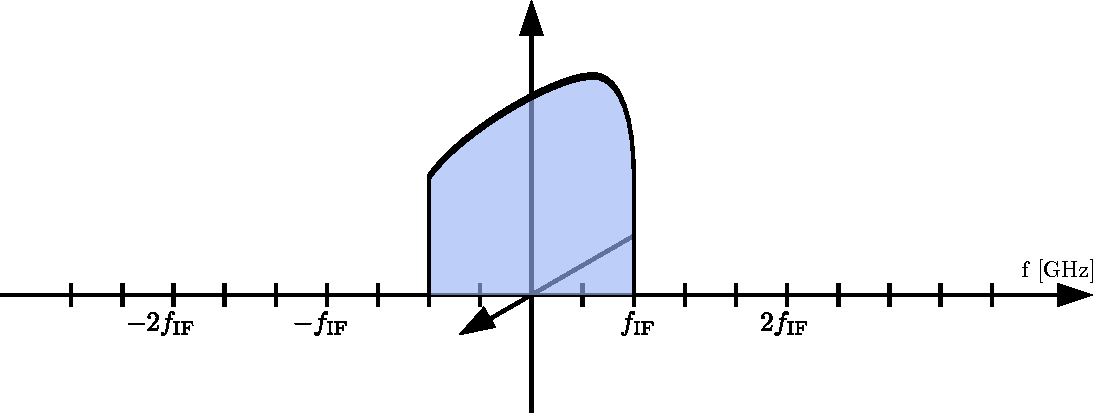
\includegraphics[width=\textwidth]{figures/rx_adc_1_freq_c}
    \caption{$c(t) = a(t) + j \cdot b(t)$}
    \label{fig:rx_adc_1_freq_c}
  \end{subfigure}
  \caption{Quadrature Baseband Mixing}
  \label{fig:rx_adc_1_freq}
\end{figure}


Self-mixing of the \gls{LO} at $f_{\text{LO}_2}$ of these mixers lead
to a \gls{DC}-offset which has to be blocked in order for the
\glspl{ADC} to work at full range.
Therefor all \glspl{ADC} are always used with \gls{DC}-blocks as described in
\secref{sec:sec:comp_dc_block}. This high-pass filters unfortunately
not only remove \gls{DC} but also a small portion of the signal
resulting in some \gls{ISI}. \\

\begin{figure}[ht]
  \centering
  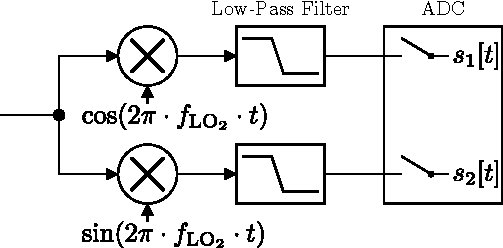
\includegraphics[width=\textwidth]{figures/rx_adc_1_bd}
  \caption{Block Diagram of Quadrature Baseband Sampling Receiver}
  \label{fig:rx_adc_1_bd}
\end{figure}

\subsection{First Nyquist-Zone Sampling}
\label{sec:rx_adc_0}
One of the simplest approach is to mix the desired signal to the first
Nyquist-zone $[0 \frac{f_s}{2}]$ of the \gls{ADC} and sample it there. \\

This results in a second \gls{IF} of $f_{\text{LO}_2} = \frac{B}{2}$ where
the sampling speed $f_s$ has to be double the bandwidth $B$.
\[f_s \geq 2 \cdot B\]

the 1.8 GHz wide signal fully falls into the first Nyquist-zone of
a single \gls{ADC} sampling at 3.6 GHz. Again a \gls{DC}-block
is used in front of the \gls{ADC}. Compared to the Quadrature Baseband
Sampling Receiver only half of the signal is lost this time since
the \gls{DC}-block now deletes the lowest frequency part of the signal
and not the central part symetrically around zero. Also this error
can be completely avoided by using a symbol rate of slighlty less
than 1.8 Ghz. \\


Hence two mixers using a \gls{LO} at $f_{\text{LO}_2} = 0.9 \text{GHz}$ are
used to downmix the signal to a quadrature baseband which than can
be sampled by two \glspl{ADC} as shown in \figref{fig:rx_0_freq_rx_if2}. \\

\begin{figure}[ht]
  \centering
  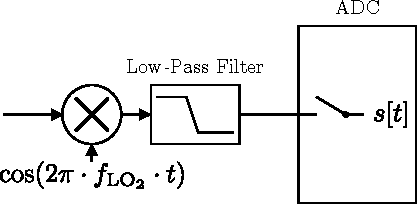
\includegraphics[width=\textwidth]{figures/rx_adc_0_bd}
  \caption{Block Diagram of First Nyquist-Zone Sampling Receiver}
  \label{fig:rx_adc_0_bd}
\end{figure}

\subsection{Sub-Nyquist Sampling}
\label{sec:rx_adc_2}

\section{Examples of Receiver Architectures}
The following secions cover three different architectures. There are example
frequencies given that are supported by the hardware available. Also their
advantages and drawbacks are disscussed. \\

\subsection{Quadrature Baseband Sampling Receiver}
\label{sec:rx_0}

The Quadrature Baseband Sampling Receiver drawn in \figref{fig:rx_0_bd}
starts with a band filter which is the same for all three architecurs
(see \figref{fig:rx_0_rf}).
It is used to minimize the total power supplied to a \gls{LNA}
Unfortenutely ajastable \gls{RF} filters are very hard to build. Therefor
the band filter is fixed to the whole band of interest. \\


\begin{figure}[ht]
  \centering
  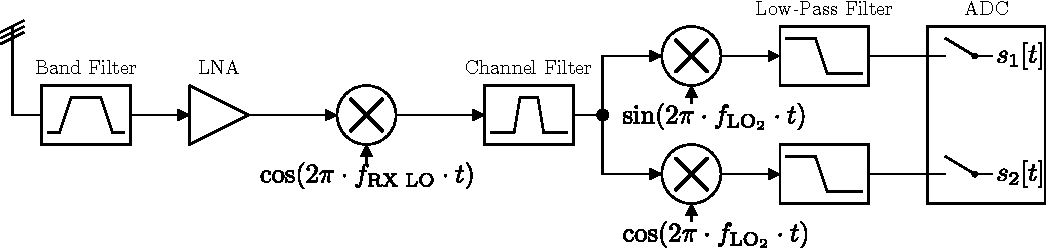
\includegraphics[width=\textwidth]{figures/rx_0_bd}
  \caption{Block Diagram of Quadrature Baseband Sampling Receiver}
  \label{fig:rx_0_bd}
\end{figure}

\begin{figure}[ht]
  \centering
  \begin{subfigure}{\textwidth}
    \centering
    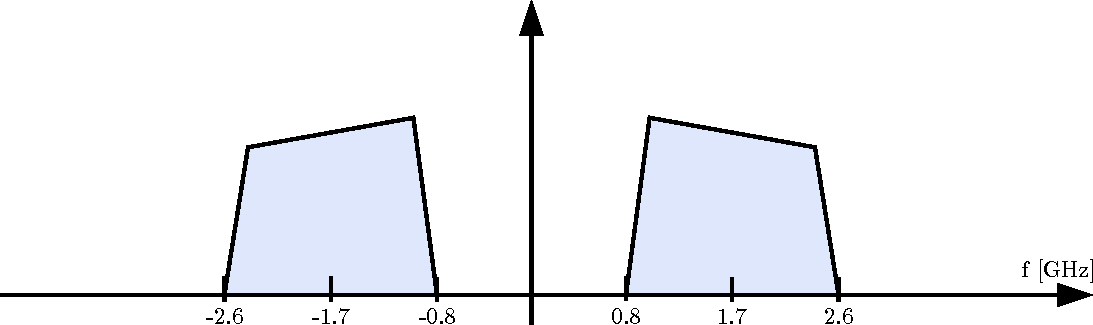
\includegraphics[width=0.8\textwidth]{figures/rx_0_freq_tx_if}
    \caption{\gls{TX} \gls{IF}}
    \label{fig:rx_0_frq_tx_if}
  \end{subfigure}
  \vspace{4ex} \\
  \begin{subfigure}{\textwidth}
    \centering
    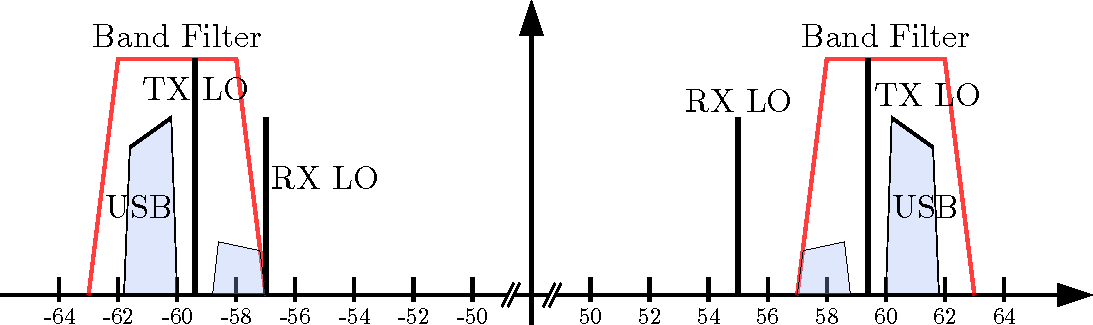
\includegraphics[width=0.8\textwidth]{figures/rx_0_freq_rf}
    \caption{\gls{RF}}
    \label{fig:rx_0_freq_rf}
  \end{subfigure}
  \vspace{4ex} \\
  \begin{subfigure}{\textwidth}
    \centering
    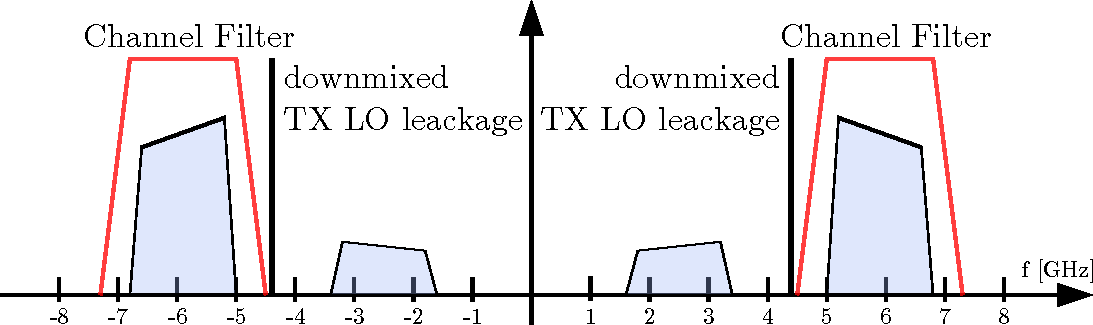
\includegraphics[width=0.8\textwidth]{figures/rx_0_freq_rx_if1}
    \caption{\gls{RX} high \gls{IF}}
    \label{fig:rx_0_freq_rx_if1}
  \end{subfigure}
  \vspace{4ex} \\
  \begin{subfigure}{\textwidth}
    \centering
    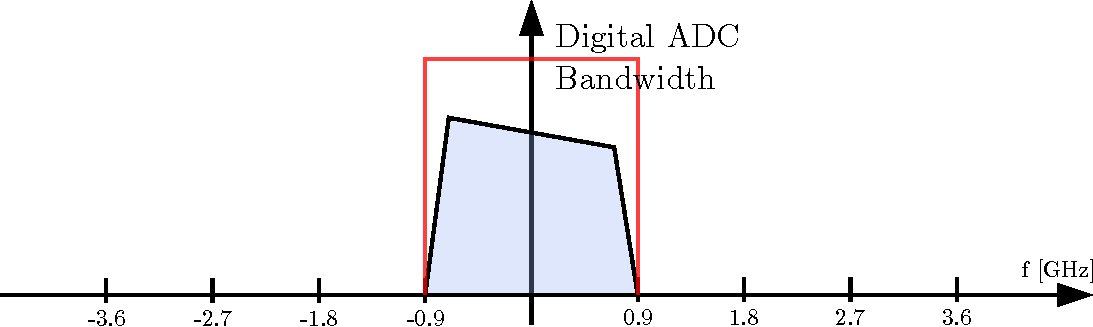
\includegraphics[width=0.8\textwidth]{figures/rx_0_freq_rx_if2}
    \caption{\gls{RX} low \gls{IF}}
    \label{fig:rx_0_freq_rx_if2}
  \end{subfigure}
  \caption{Quadrature Baseband Sampling Receiver in Frequency Domain}
  \label{fig:rx_0_freq}
\end{figure}

\subsection{Intermediate Frequency Sampling Receiver}
\label{sec:rx_1}
Next a different receiver architecture was considered which uses
two mixer paths to mix the signal and it's $90^\circ$ shifted version
from \gls{RF} to the first \gls{IF} and are than combined using
a second $90^\circ$ coupler resulting in the \gls{RX} \gls{LSBand}
to be suppressed.
This allows for a lower \gls{IF} (see \figref{fig:rx_1_bd}).
As decribed in \secref{sec:rx_0} the \gls{IF} of the
Quadrature Baseband Sampling Receiver had a lower bound due to the needed
separation of the \gls{RX} side bands. \\

The channel selection was than done by a high-pass filter before
the second mixer removing all signals between $f_{\text{RX LO}}$ and
$f_{\text{c}} - \frac{B}/{2}$ including the strong \gls{TX} \gls{LO}
leackage. \\

The second \gls{IF} of $f_{\text{LO}_2} = 0.9$ was assigned such that
the 1.8 GHz wide signal fully falls into the first Nyquist-zone of
a single \gls{ADC} sampling at 3.6 GHz. Again a \gls{DC}-block
is used in front of the \gls{ADC}. Compared to the Quadrature Baseband
Sampling Receiver only half of the signal is lost this time since
the \gls{DC}-block now deletes the lowest frequency part of the signal
and not the central part symetrically around zero. Also this error
can be completely avoided by using a symbol rate of slighlty less
than 1.8 Ghz. \\

A drawback of this architecture is, that it requires a single \gls{ADC}
at the symbol speed $f_{s}$ instead of two \gls{ADC} channels at
$f_{s} / s$ used by the two other architectures. Such \gls{ADC} can,
as it was done in our setup, be build using a two channel \gls{ADC}
in interleaved mode. This may introduce many new errors as the not
perfect balancing of both channels and a high clock jitter frequency
component at $f_{s}$. \\

\begin{figure}[ht]
  \centering
  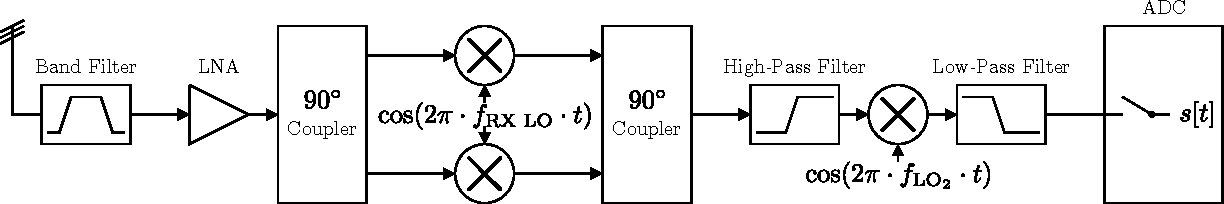
\includegraphics[width=\textwidth]{figures/rx_1_bd}
  \caption{Block Diagram of Intermediate Frequency Sampling Receiver}
  \label{fig:rx_1_bd}
\end{figure}

\begin{figure}[ht]
  \centering
  \begin{subfigure}{\textwidth}
    \centering
    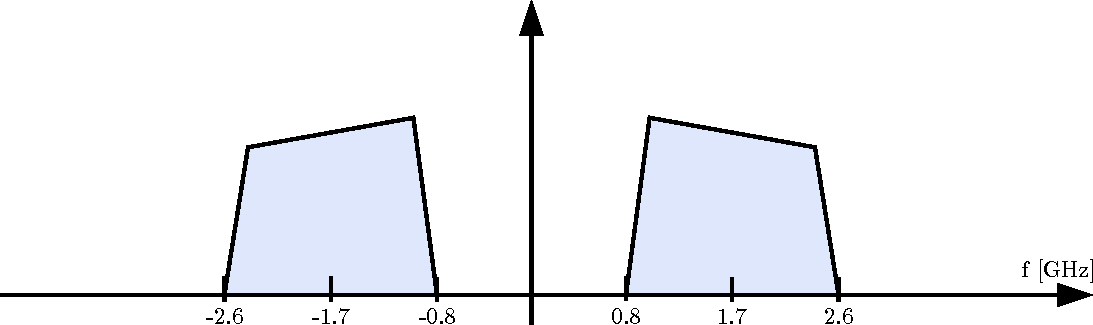
\includegraphics[width=0.8\textwidth]{figures/rx_1_freq_tx_if}
    \caption{\gls{TX} \gls{IF}}
    \label{fig:rx_1_frq_tx_if}
  \end{subfigure}
  \vspace{4ex} \\
  \begin{subfigure}{\textwidth}
    \centering
    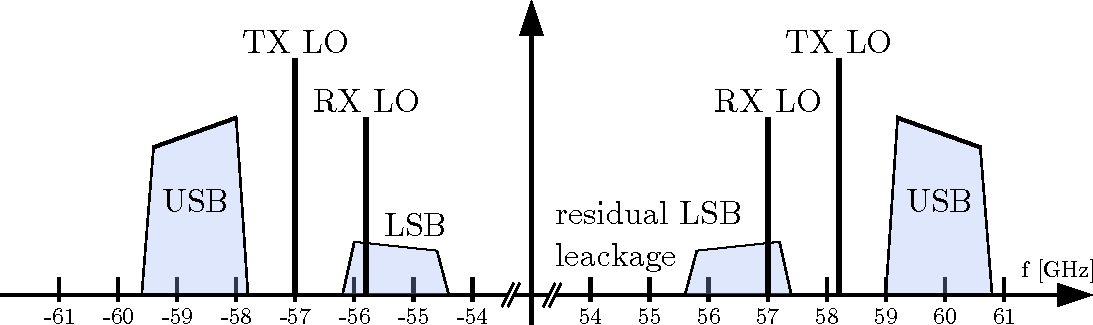
\includegraphics[width=0.8\textwidth]{figures/rx_1_freq_rf}
    \caption{\gls{RF}}
    \label{fig:rx_1_freq_rf}
  \end{subfigure}
  \vspace{4ex} \\
  \begin{subfigure}{\textwidth}
    \centering
    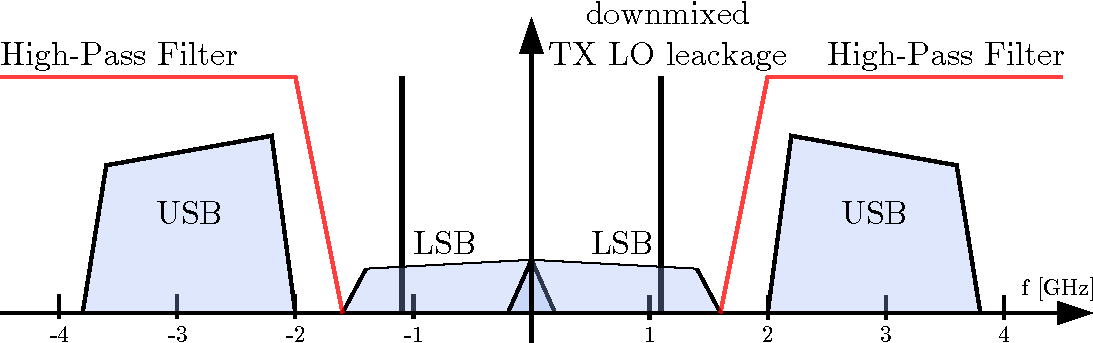
\includegraphics[width=0.8\textwidth]{figures/rx_1_freq_rx_if1}
    \caption{\gls{RX} high \gls{IF}}
    \label{fig:rx_1_freq_rx_if1}
  \end{subfigure}
  \vspace{4ex} \\
  \begin{subfigure}{\textwidth}
    \centering
    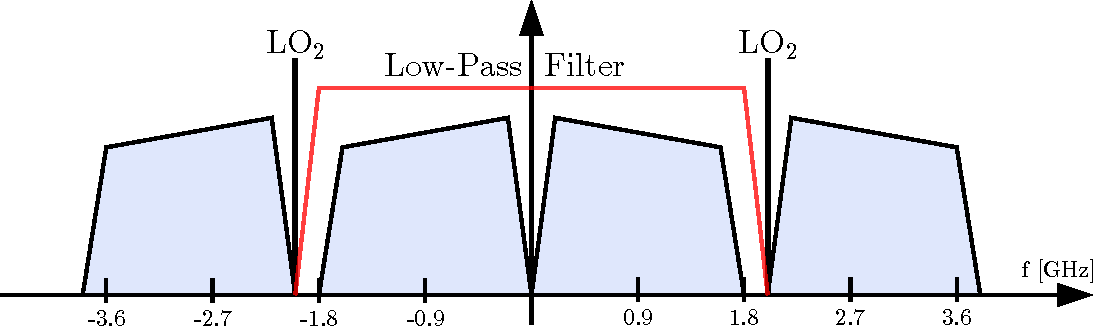
\includegraphics[width=0.8\textwidth]{figures/rx_1_freq_rx_if2}
    \caption{\gls{RX} low \gls{IF}}
    \label{fig:rx_1_freq_rx_if2}
  \end{subfigure}
  \caption{Intermediate Frequency Sampling Receive in Frequency Domain}
  \label{fig:rx_1_freq}
\end{figure}

\subsection{Quadrate Intermediate Frequency Sub-Nyquist Sampling Receiver}
Assumption that no signal on neighbouring channels. \\

Finally we came up with a third receiver architecture only using very
few components which add non-linearities. \\

The basic idea

Since the to mixers located in front of the \gls{ADC} work at much
higher frequencies than those used in the other architectures the
\gls{LO}-leackage and it's self-mixing is even more pronounced.
Therefor used


\begin{itemize}
\item USB / LSB problem similar to IF-Mixer image suppression
\item Problem can be solved by using only one mixer and quadrature sampling.
\item Needs double the bandwidth to sample both channels with the full
  signal bandwidth
\item Use sub-nyquist sampling to avoid DC-offset problem and low-frequency
  limitation of components (carrier leakage)
\item Only very few components needed -> less non-idealities
\item since mixer works at much high frequencies than the second mixer of
  previous architectures, much bigger LO-leackage -> cannot work down to DC
\end{itemize}

\begin{figure}[ht]
  \centering
  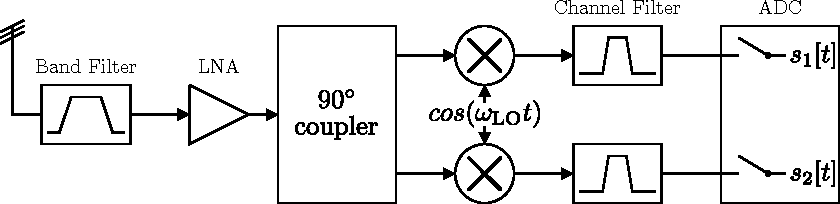
\includegraphics[width=\textwidth]{figures/quad_if_rx_block_diagram}
  \caption{Block Diagram of Quadrate Intermediate Frequency Sub-Nyquist Sampling Receiver}
  \label{fig:rx_2_bd}
\end{figure}

\begin{figure}[ht]
  \centering
  \begin{subfigure}{\textwidth}
    \centering
    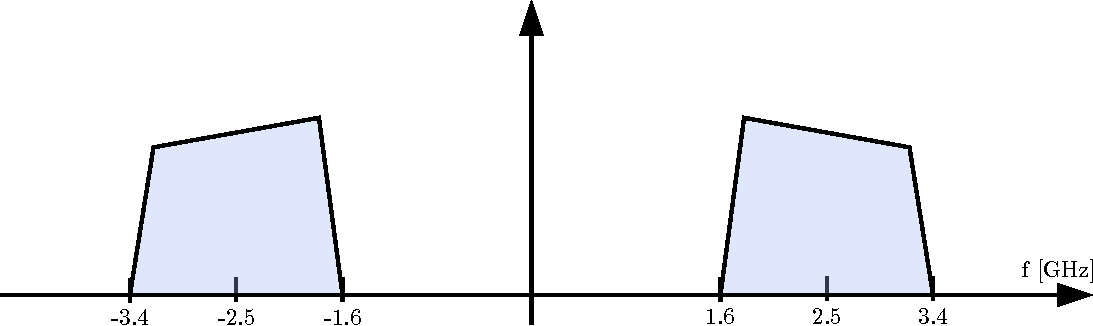
\includegraphics[width=0.8\textwidth]{figures/rx_2_freq_tx_if}
    \caption{\gls{TX} \gls{IF}}
    \label{fig:rx_2_frq_tx_if}
  \end{subfigure}
  \vspace{4ex} \\
  \begin{subfigure}{\textwidth}
    \centering
    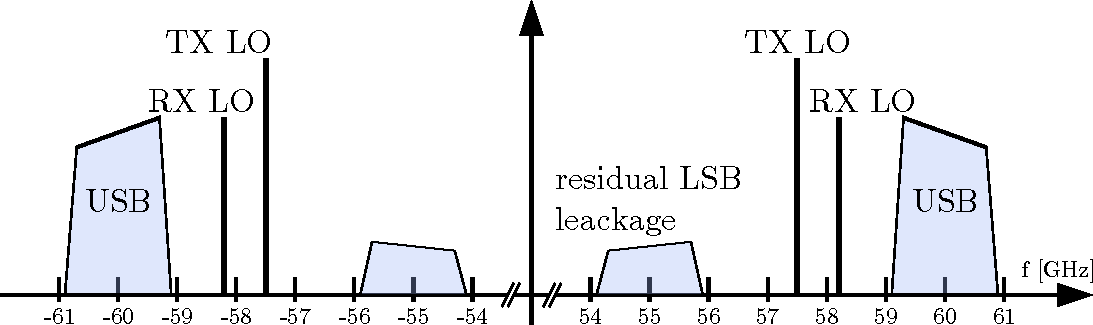
\includegraphics[width=0.8\textwidth]{figures/rx_2_freq_rf}
    \caption{\gls{RF}}
    \label{fig:rx_2_freq_rf}
  \end{subfigure}
  \vspace{4ex} \\
  \begin{subfigure}{\textwidth}
    \centering
    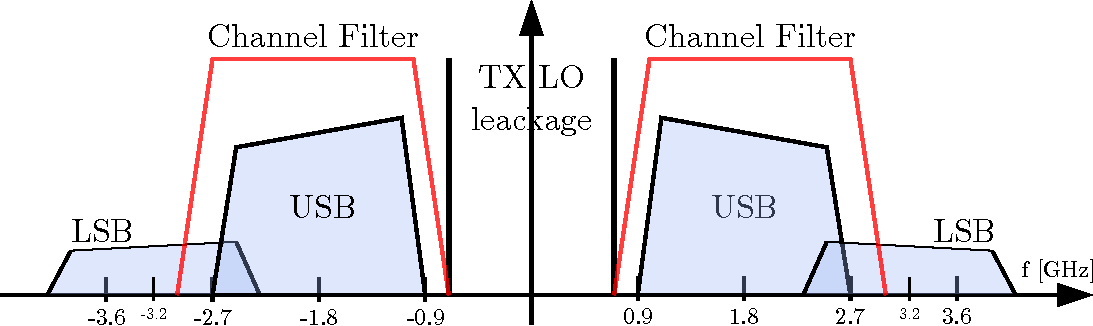
\includegraphics[width=0.8\textwidth]{figures/rx_2_freq_rx_if}
    \caption{\gls{RX} \gls{IF}}
    \label{fig:rx_2_freq_rx_if1}
  \end{subfigure}
  \vspace{4ex} \\
  \begin{subfigure}{\textwidth}
    \centering
    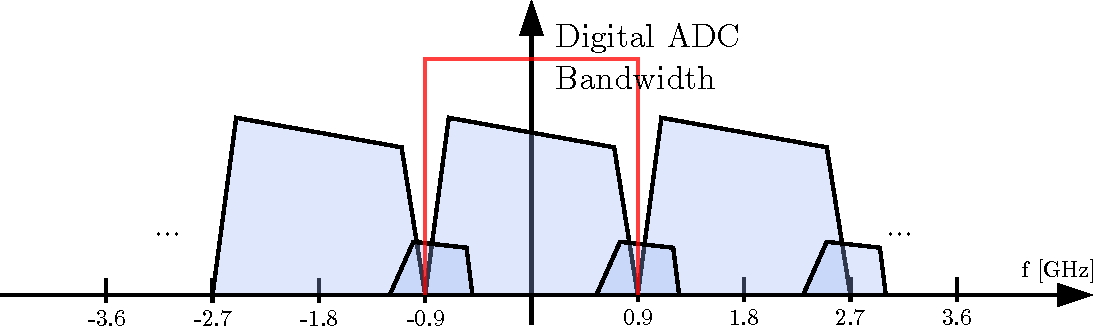
\includegraphics[width=0.8\textwidth]{figures/rx_2_freq_rx_adc}
    \caption{Sampled Signal}
    \label{fig:rx_2_freq_rx_if2}
  \end{subfigure}
  \caption{Quadrate Intermediate Frequency Sub-Nyquist Sampling Receiver
    in Frequency Domain}
  \label{fig:rx_2_freq}
\end{figure}
